\documentclass[11pt]{beamer}
\usetheme{CambridgeUS}
\usepackage[utf8]{inputenc}
\usepackage[english]{babel}
\usepackage{amsmath}
\usepackage{amsfonts}
\usepackage{amssymb}
\usepackage{graphicx, subfig}
\usepackage{booktabs}

\author{Carlo Alessi \& Doria Saric}
\title{Extraction of Drug-Drug Interactions from Biomedical Texts}
%\setbeamercovered{transparent} 
%\setbeamertemplate{navigation symbols}{} 
%\logo{} 
%\institute{} 
%\date{} 
%\subject{} 

\begin{document}
\AtBeginSection[]
{
 \begin{frame}<beamer>
 \frametitle{Outline}
 \tableofcontents[currentsection]
 \end{frame}
}

\begin{frame}
\titlepage
\end{frame}

%\begin{frame}
%\tableofcontents
%\end{frame}

\section{Software}
\begin{frame}{Software}
\begin{itemize}
\item Base language: Python
\item XML parser: ElementTree
\item Pandas
\item Numpy
\item Gensim: Word2Vec
\item NLTK
\begin{itemize}
\item[a.] Word tokenizer
\item[b.] Part-of-Speech tagger
\item[c.] English stemmer
\end{itemize}
\item Scikit Learn
\begin{itemize}
\item[a.] Data preprocessing
\item[b.] Pipelines
\item[c.] SVM
\end{itemize}
\item Keras: ANN
\end{itemize}
\end{frame}

\begin{frame}{Method}
\begin{itemize}
\item Task9.1 -- 2 approaches
\begin{itemize}
	\item[a.] Embeddings: stemming, POS, puctuation removal, lowercase
	\item[b.] Hand-crafted features:\\
	\begin{itemize}
		\item Is the word capitalized?
		\item Is the part of speech NN?
		\item Previous word, following word -- word2vec
		\item If there are some \textbf{trigger} words surrounding this word?
		\item Does the word have more consonants than vocals?
	\end{itemize}
	%\item[c.] (a) and (b) combined
\end{itemize}
\item Task9.2
\begin{itemize}
\item Hierarchical classification (binary + multiclass)
\end{itemize}
\end{itemize}
\end{frame}

\section{Learners}
\begin{frame}{Learners}
\begin{itemize}
\item Training/Validation split: $(90\%,10\%) \sim (133k, 14k)$ words 
\item Metrics:
\item[1.] Feed-forward Neural Network
\begin{itemize}
\item Architecture: $[vector\_size, 512, 256, 128, 3]$
\item Activations: ReLU, Softmax
\item Dropout fraction: 0.5
\item Objective: Categorical cross-entropy
\item Solver: Adam
\item Number of parameters: 175363
\end{itemize}
\item[2.] Support Vector Machine
\begin{itemize}
\item Kernel: radial basis function
\item $C=1$
\item $\gamma = auto$
\item $\alpha = 0.001$
\end{itemize}
\end{itemize}
\end{frame}

\section{Experiments}
\subsection{Word Vectors}
\begin{frame}{Word Vectors}

\begin{columns}
\begin{column}{0.25\textwidth}
\begin{itemize}
\item Vector size
\item Vector type
\item Preprocessing
\end{itemize}
\end{column}

\begin{column}{0.75\textwidth}
\begin{table}
\centering
\resizebox{0.5\columnwidth}{!}{%
\begin{tabular}{ccc}
\toprule
Vector size & Micro F1	& Macro F1 \\
\midrule
10 &	0.9481 & 0.5041	\\
\textbf{20} &	\textbf{0.9517} & \textbf{0.5435}	\\	
50 &	0.9495	& 0.5215	\\
100 &	0.9499	& 0.5232	\\
200 &	0.9479	& 0.4855	\\
\bottomrule
\end{tabular}
}
\caption{F1-score for different word-vector sizes.}
\end{table}
\begin{table}
\centering
\resizebox{0.5\columnwidth}{!}{%
\begin{tabular}{ccc}
\toprule
Type	&	Micro f1 & Macro f1 \\
\midrule
original &	0.9499	& 0.5098	\\
\textbf{stem}	&	\textbf{0.9599}	& \textbf{0.6144}	\\
original + PoS	 & 0.9481 & 0.5105	\\
stem + PoS	& 0.9517 & 0.5435	\\
\bottomrule
\end{tabular}
}
\caption{F1-score for different word-vector types.}
\end{table}
\end{column}
\end{columns}
\end{frame}


\begin{frame}{Word Vectors}

\begin{columns}
\begin{column}{0.25\textwidth}
\begin{itemize}
\item Vector size
\item Vector type
\item Preprocessing
\end{itemize}
\end{column}

\begin{column}{0.75\textwidth}
\begin{table}
\parbox{.5\columnwidth}{
\begin{tabular}{ccc}
\toprule
Preprocessing &	Micro f1 & Macro f1	\\
\midrule
No    &   0.9599	& 0.6144	\\
Minmax(0,1) &	0.9515	& 0.5207	\\
Standardize &	0.9581  & 0.5897	\\
\bottomrule
\end{tabular}
\caption{F1-score for different preprocessing.}
}
\end{table}
\end{column}
\end{columns}
\end{frame}


\subsection{Learning curves}
\begin{frame}{Loss/Accuracy}

\begin{figure}
\subfloat[loss]{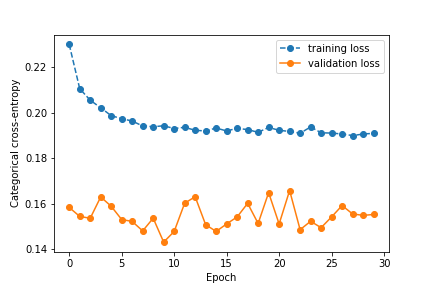
\includegraphics[width=0.5\columnwidth]{./images/loss.png}}
\subfloat[accuracy]{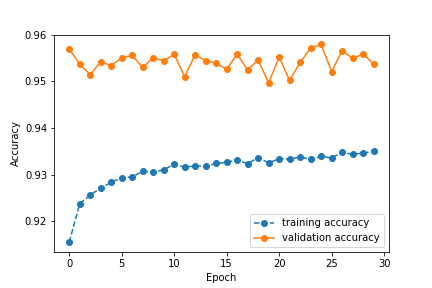
\includegraphics[width=0.5\columnwidth]{./images/accuracy.png}}
\caption{Learning curves}
\end{figure}

\end{frame}

\begin{frame}{Micro F1/Precision/Recall score}
\begin{figure}
\center
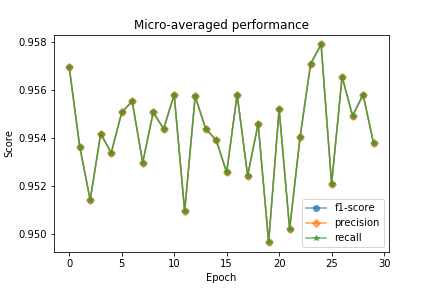
\includegraphics[width=0.8\columnwidth]{./images/micro.png}
\caption{Micro scores.}
\end{figure}
\end{frame}

\begin{frame}{Macro/Weighted F1/Precision/Recall score}
\center
\begin{figure}
\subfloat[loss]{
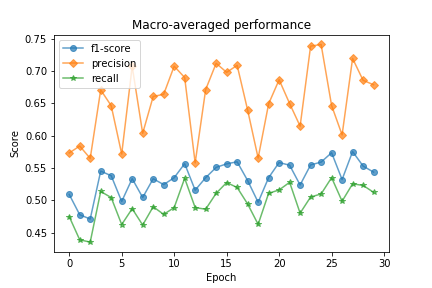
\includegraphics[width=0.5\columnwidth]{./images/macro.png}
}
\subfloat[accuracy]{
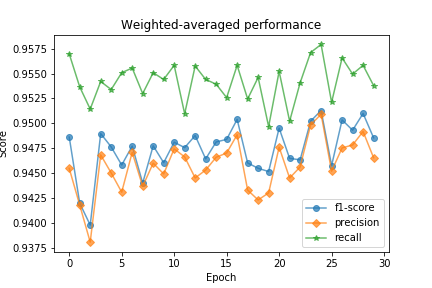
\includegraphics[width=0.5\columnwidth]{./images/weighted.png}
}
\caption{Macro and Weighted scores.}
\end{figure}
\end{frame}

\section{Results}
\begin{frame}{Results}
\begin{table}
\begin{tabular}{c|ccc|ccc}
\toprule
& \multicolumn{3}{c}{Exact} & \multicolumn{3}{c}{Partial}\\
\midrule
& Precision & Recall & F1 & Precision & Recall & F1\\
\midrule
DrugBank & 0.61 &	0.43	& 0.5 & 0.61	& 0.5 &	0.55\\
MedLine & 0.51	& 0.29 & 0.37 & 0.51	& 0.35 &	0.41\\
Both& 0.56	& 0.35	& 0.43	& 0.56	& 0.41	& 0.48\\
\bottomrule
\end{tabular}
\caption{Results Task1 on gold test dataset.}
\end{table}
\end{frame}

\section{Conclusions}
\begin{frame}{Conclusions}
\begin{itemize}
\item Word vector size (too small, too big)
\item stemming and PoS improved performance used individually, but not in conjuction
\item Poor results (especially the recall)
\begin{itemize}
\item Poor features?
\item Limited model capacity/expressivess?
\end{itemize}
\end{itemize}
\end{frame}

\end{document}